\documentclass{article}
\usepackage[utf8]{inputenc}
\usepackage[T1]{fontenc}
\usepackage{graphicx}
\usepackage{hyperref}
\usepackage{geometry}
\geometry{margin=1in}

\title{ENDYMON}
\date{Encyclopaedia Britannica (1771)}

\begin{document}
\maketitle

\section*{Historical source}
\textbf{Entry ID:} \texttt{entry-endymon-523} \\
\textbf{Volume ID:} 144850375 \\
\textbf{Character Count:} 378

\subsection*{Extracted Text}
ENDYMON, the 1zth king of Elia. Being ex- pelled his kingdom, he retired into Caria to mount Lat-mos, where he fluded the bewenly bodies, but chiefly the moo's which gave rise to the false of the poets, that he was beloved by the moo, who visited him every night as he lay alleep upon the top of that hill.

ENEM In law, an alien or foreigner, who pub- lied invades the kingdom.



\section*{Source record}
\begin{itemize}
\item \textbf{Dataset:} \texttt{NationalLibraryOfScotland/encyclopaedia\_britannica\_illustrated}
\item \textbf{Dataset Revision:} \texttt{309f765b1ecc83e0a7f7762e44b4a927a7555443}
\item \textbf{Page ID:} \texttt{britannica:309f765b1ecc83e0a7f7762e44b4a927a7555443:train:523} \\
  \textbf{Filename:} \texttt{page-0523-a583606e375a.jpg} \\
  \textbf{Row Index:} 523 \\
  \textbf{SHA256:} \texttt{a583606e375ad92d...}
\end{itemize}

\begin{figure}[h]
\centering
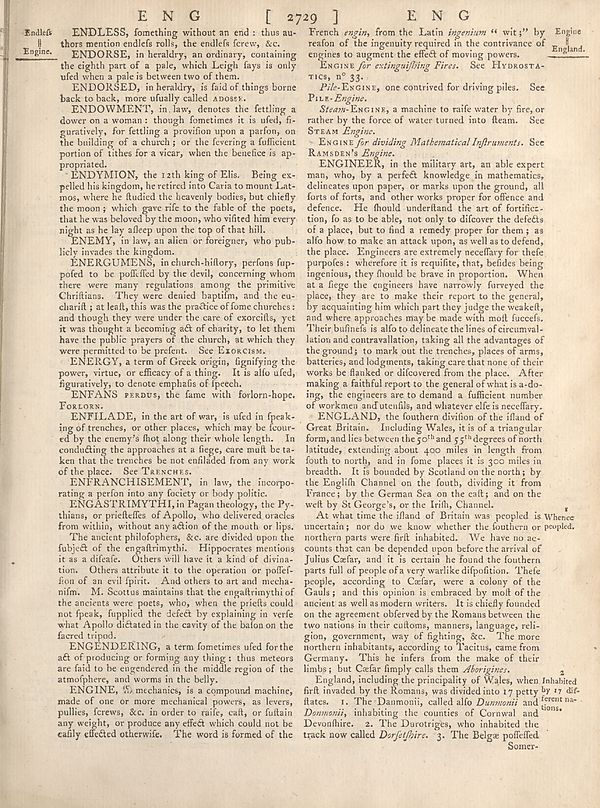
\includegraphics[width=0.85\textwidth]{../scans/page-0523-a583606e375a.jpg}
\caption*{Source scan: \texttt{page-0523-a583606e375a.jpg}}
\end{figure}

\end{document}
